% 2 Oort-Lindbladモデルと観測方程式 (仮)
% 2.1 速度分散の無い系の太陽運動と銀河速度場 ← 宮本ノートや藤田修論を参考に書く
% 2.1.1 Oort-Lindbladモデル ← A, B, C, Kの導出と物理的意味
% 2.1.2 観測方程式 ← 従来のもの

% 2.2 速度分散を考慮した場合への拡張 ← Olling & Dehnenを参考に書く
% 2.2.1 従来のOort-Lindbladモデルの問題点 ← ここにYu & Liu の年齢速度分散関係の図も載せるとよい。
% 2.2.2 asymmetric drift ← 導出&物理的解釈を書く
% 2.2.3 asymmetric driftを考慮した観測方程式



% Chap. 2 Oort-Lindbladモデルと観測方程式
% p.11にOlling & Dehnen 2002の表 (A, B, C, Kの表記の違い) を載せていますが、
% この表記の表は載せる必要がありますか?

% 式(2.30a,b)の導出と、それを用いたAa, Baとvaの関係の評価 (すぐ下に文章で書いてある) は、
% 単にOlling & Dehnenの翻訳ではなく、ちゃんと自分の言葉で書きましょう。
% (そもそもここの文章に書いてある近似式は自分で導出しましたか?)
% この関係は、模擬データの解析結果の解釈の部分でも利用する近似式だと思います。


\chapter{Oort-Lindbladモデルと観測方程式 \label{chapTheory}}
この章では、本研究で用いているOort-Lindbladモデルと、実際に観測データにこのモデルを適用する観測方程式の説明をする。まず、速度分散の無い系でのOort-Lindbladモデルと観測方程式について説明する。その後、従来のOort-Lindbladモデルの問題点と、速度分散を考慮した場合に考えるべき効果に加えて、そのような場合に拡張した観測方程式の説明をする。

ここで、本章で用いる文字の表記法を表整理しておく。
\begin{table}
\begin{center}
%\scalebox{0.5}
%\scriptsize
%\footnotesize
%\small
\begin{tabular}{c|l} \hline
 \rowcolor{LightCyan}
 文字 & 文字が示す意味\\
 \hline
 $\pmb{R}$ & 銀河中心を基準とした星の位置ベクトル\\
 \hline
 $\pmb{R_{\odot}}$ & 銀河中心を基準とした太陽の位置ベクトル\\
 \hline
 $\pmb{r}$ & 太陽に対する星の位置ベクトル ($\pmb{r}=\pmb{R}-\pmb{R_{\odot}}$)\\
 \hline
 $\pmb{v}_*$ & 銀河中心から見た星の速度\\
 \hline
 $\pmb{v}_{\odot}$ & 銀河中心から見た太陽の速度\\
 \hline
 $\pmb{V}(\pmb{R})$ & 速度分散があるときの銀河中心から見た位置$\pmb{R}$での系統速度\\
 \hline
 $\pmb{V}_{\mathrm{c}}(\pmb{R})$ & 速度分散がない、すなわち星が円軌道のときの銀河中心から見た位置$\pmb{R}$での系統速度\\
 \hline
 $\pmb{v}_{\mathrm{p}}$ & 星の特異速度\\
 \hline
 $\pmb{v}_{\mathrm{p},\odot}$ & 太陽の特異速度\\
 \hline
 $\pmb{v}_{\mathrm{rel}}$ & 太陽から見たときの星の速度\\
 \hline
 $x、y$ & 太陽を中心とした直交座標系におけるそれぞれ銀経$l=0^{\circ}、90^{\circ}$の向きの座標\\
 \hline
 $\sigma_R、\sigma_{\phi}、\sigma_z$ & 円筒座標系で表された速度の速度分散\\
 \hline
 \multirow{2}{*}{$A、B、C、K$} & 星が閉じた軌道で運動しているときのオールト定数。\\
    & それぞれ銀河回転方向の剪断成分、回転成分、動径成分、発散成分。 \tabularnewline[\doublerulesep] 
 \hline
 \multirow{2}{*}{$\overline{A}、\overline{B}、\overline{C}、\overline{K}$} & 星が閉じていない軌道で運動しているときの平均速度場のオールト定数。\\
   & それぞれ銀河回転方向の剪断成分、回転成分、動径成分、発散成分。 \tabularnewline[\doublerulesep] 
 \hline
 $U_{\odot}、V_{\odot}、W_{\odot}$ & 太陽の特異速度の動径方向、銀河回転方向、銀河北極方向成分\\
 \hline
 $U_{\odot}、V_{\odot}、W_{\odot}$ & 太陽の特異速度の動径方向、銀河回転方向、銀河北極方向成分\\
 \hline
 $(R,\phi,z)$ & 銀河中心を中心とした円筒座標系\\
 \hline
 $(R,\theta,\phi)$ & 銀河中心を中心とした球対称座標系\\
 \hline
 $\Phi$ & 重力ポテンシャル\\
 \hline
\end{tabular} \label{notation}
\vspace{3mm}
\caption{模擬データ生成で用いた年齢と速度分散の対応表 (\cite{YL18})。速度分散は銀河中心を中心とした円筒座標系$(R,\phi,z)$となっている。}
\end{center}
\end{table}

\section{速度分散の無い系の太陽運動と銀河速度場} % 宮本ノートや藤田修論を参考に書く
この節では、速度分散の無い系での太陽運動とOort-Lindbladモデル、銀河系の速度場について説明する。太陽系近傍の星の速度は、系統速度 (streaming velocity) と特異速度 (peculiar velocity) とに分けることができ、太陽運動とは太陽の特異速度のことを意味する。系統速度とは、銀河系内のある位置でのある一意な速度のことである。特異速度とは、系統速度と1つ1つの星の速度との差であり、銀河系の星は基本的には円軌道ではないため、それぞれの星ごとそれぞれの特異速度を持つ。太陽位置を系統速度で動く点は局所静止基準 (LSR; Local Standard of Rest) と呼ばれ、太陽系の位置で銀河系中心を中心として円運動をする仮想的な点で考えられる。本論文では、太陽運動は$\pmb{v}_{\mathrm{p},\odot} = (U_{\odot},V_{\odot},W_{\odot})$で表す。$(U_{\odot},V_{\odot},W_{\odot})$はそれぞれ銀河中心方向、銀河回転方向、銀河北極方向と定義する (図\ref{fig:SolarMotion})。
\begin{figure*}[htbp]
\begin{center}
	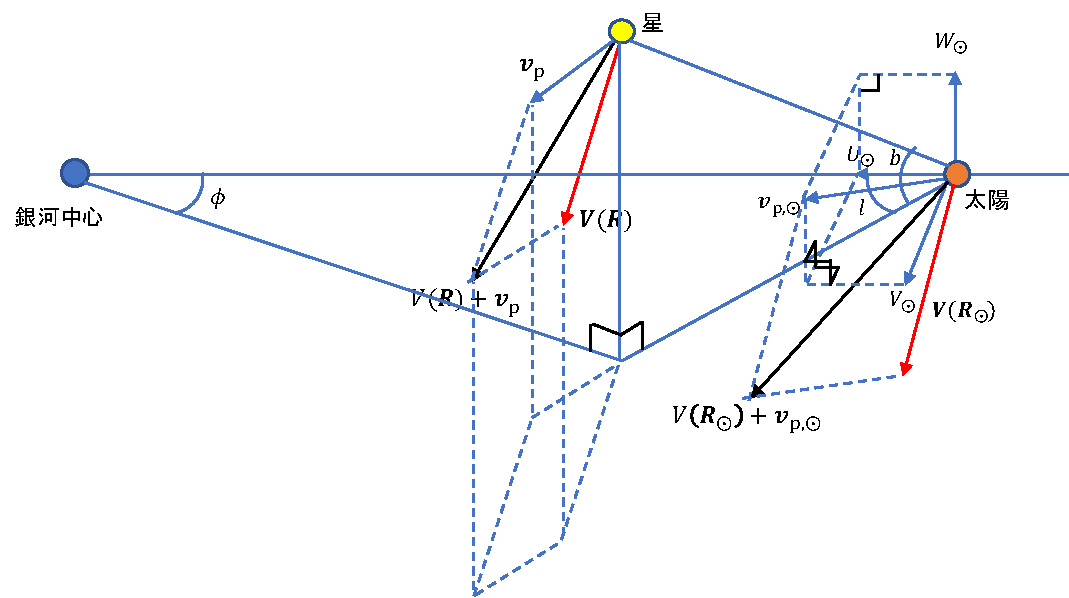
\includegraphics[width=10cm]{fig/SolarMotion.pdf}
	\caption{太陽運動$(U_{\odot},V_{\odot},W_{\odot})$の向き。それぞれ銀河中心方向、銀河回転方向、銀河北極方向のベクトルであり、直交座標系に沿ったベクトルである。}
	\label{fig:SolarMotion}
\end{center}
\end{figure*}

%%%%%%%%%%%%%%%%%%%%%%%%%%%%%%%%%%%%%%%%%%%%%%%%%%%%%%%%%%%%%%%%%%%%%%%%
%%%%%%%%%%%%%%%%%%%%%%%%%%%%%%%%%%%%%%%%%%%%%%%%%%%%%%%%%%%%%%%%%%%%%%%%
%%%%%%%%%%%%%%%%%%%%%%%%%%%%%%%%%%%%%%%%%%%%%%%%%%%%%%%%%%%%%%%%%%%%%%%%

\subsection{Oort-Lindbladモデル} % A, B, C, Kの導出と物理的意味
Oort-Lindbladモデルとは、\cite{Oort1927b}, \cite{Lindblad1927}, \cite{Chandra42}らによって構築された太陽近傍の銀河系速度場を記述するモデルである。ここでは、このモデルの導出とパラメータの説明をする。

銀河系中心に原点を置く静止座標系を考える。このときの太陽近傍星と太陽の速度をそれぞれ$\pmb{v}_{*}、\pmb{v}_{\odot}$とする。また、位置$\pmb{R}$での系統速度を$\pmb{V}(\pmb{R})$、太陽近傍星と太陽の特異速度をそれぞれ$\pmb{v}_{\mathrm{p}}、\pmb{v}_{\mathrm{p}_\odot}$とする (図\ref{fig:motion})。
\begin{figure*}[htbp]
\begin{center}
	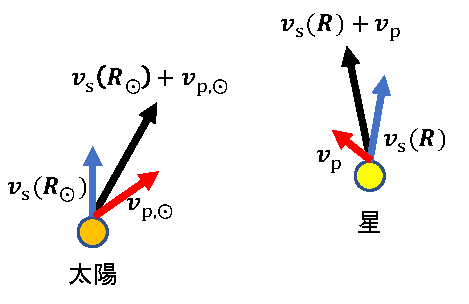
\includegraphics[width=7cm]{fig/motion.pdf}
	\caption {星と太陽の系統速度$\pmb{V}(\pmb{R})、\pmb{V}(\pmb{R_{\odot}})$、星と太陽の特異速度$\pmb{v}_{\mathrm{p}}、\pmb{v}_{\mathrm{p}_\odot}$をベクトルで書いたときの例。図のように速度ベクトルを足すことで、銀河中心に対する星の速度は$\pmb{V}(\pmb{R}_{\odot}) + \pmb{v}_{\mathrm{p},\odot}$、銀河中心に対する太陽の速度は$\pmb{V}(\pmb{R}) + \pmb{v}_{\mathrm{p}}$と表せる。}
	\label{fig:motion}
\end{center}
\end{figure*}
また、2次元面 (銀河円盤面) に運動を限定する。すなわち、銀緯$b=0^{\circ}$の面で考える。このとき、
\begin{align}
\begin{aligned}
	\pmb{v}_* &= \pmb{V}(\pmb{R}) + \pmb{v}_{\mathrm{p}} \\
	\pmb{v}_{\odot} &= \pmb{V}(\pmb{R}_{\odot}) + \pmb{v}_{\mathrm{p},\odot}
\end{aligned}
\end{align}
と書ける。太陽から見たときの太陽近傍星の速度$\pmb{v}_{\rm rel}$は、星の特異速度を無視すると、
\begin{align}
\begin{aligned}
	\pmb{v}_{\rm rel} &= \pmb{v}_* - \pmb{v}_{\odot} \\
	&= [\pmb{V}(\pmb{R}) - \pmb{V}(\pmb{R}_{\odot})] - \pmb{v}_{\mathrm{p},\odot}
\end{aligned}
\end{align}
となる。ここで、太陽に対する星の位置ベクトルを$\pmb{r} = \pmb{R} - \pmb{R}_{\odot}$とする。$\pmb{R}、\pmb{R}_{\odot}$はそれぞれ星、太陽の位置ベクトルである。星と太陽との距離が星と銀河中心との距離$\pmb{x}$に対して十分小さい$(|\pmb{r}| = |\pmb{R}-\pmb{R}_{\odot}| \ll |\pmb{x}|)$と仮定すると、太陽にいる観測者から見た銀河系内でのある位置$\pmb{R}$での系統速度はテイラー展開することができる。このとき、太陽を中心とした直交座標系を考え、$x$軸、$y$軸はそれぞれ銀経$l=0^{\circ}、90^{\circ}$の方向とすると、
\begin{align}
\begin{aligned}
	\pmb{v}_{\rm rel} &\simeq \pmb{H} \cdot \pmb{r} - \pmb{v}_{\mathrm{p},\odot} + \mathcal{O}(\pmb{r}^2) \label{eq:1}
\end{aligned}
\end{align}
と書けるから、
\begin{align}
\begin{aligned}
	\pmb{H} \simeq
	\left. \frac{\partial \pmb{V}(\pmb{R})}{\partial \pmb{R}} \right|_{\pmb{R}=\pmb{R}_{\odot}}
	&=
	\left(
	\begin{array}{cc}
	 	\cfrac{\partial V_x}{\partial x} & \cfrac{\partial V_x}{\partial y}\\
		\cfrac{\partial V_y}{\partial x} & \cfrac{\partial V_y}{\partial y}\\
	\end{array}
	\right) \\
	&=
	\left(
	\begin{array}{cc}
	 	K+C & A-B\\
		A+B & K-C\\
	\end{array}
	\right)
\end{aligned} \label{eq2}
\end{align}
となる。ここで、$A、B、C、K$を以下のように定義すると
\begin{subequations}
\begin{align}
	A &=\frac{1}{2}\left(\frac{\partial V_y}{\partial x} + \frac{\partial V_x}{\partial y}\right) \label{eq2.1a}\\
	B &=\frac{1}{2}\left(\frac{\partial V_y}{\partial x} - \frac{\partial V_x}{\partial y}\right) \label{eq2.1b}\\
	C &=\frac{1}{2}\left(\frac{\partial V_x}{\partial x} - \frac{\partial V_y}{\partial y}\right) \label{eq2.1c}\\
	K &=\frac{1}{2}\left(\frac{\partial V_x}{\partial x} + \frac{\partial V_y}{\partial y}\right) \label{eq2.1d}
\end{align} \label{eq2.1}
\end{subequations}
となる。

パラメータ$A,B,C,K$はオールト定数と呼ばれる。これらは太陽近傍星の運動学が力学的に冷たい系である場合の平均速度場を表すパラメータであり、それぞれ銀河回転方向の剪断成分、回転成分、動径(太陽と銀河中心を結ぶ方向)成分、発散成分を示す。式(\ref{eq2.1})は直交座標系で表したオールト定数であるが、一般的にはオールト定数は円筒座標系$(R,\phi)$(座標系の取り方は図(\ref{fig:coordinates})を参照)で表される(\cite{Chandra42})。そこで、直交座標系から円筒座標系への座標変換をする。
\begin{align}
\begin{cases}
	x &= R_{\odot} - R\cos{\phi}\\
	y &= R\sin{\phi}
\end{cases}
\end{align}

\begin{align}
\begin{cases}
	R &= \sqrt{(R_{\odot}-x)^2 + y^2 }\\
	\phi &= \arctan{\cfrac{y}{R_{\odot}-x}}
\end{cases}
\end{align}

\begin{align}
\begin{aligned}
	\left(
	\begin{array}{c}
	 	V_x\\
		V_y\\
	\end{array}
	\right)
	&=
	\left(
	\begin{array}{cc}
	 	\cos{\phi} & \sin{\phi}\\
		-\sin{\phi} & \cos{\phi}\\
	\end{array}
	\right)
	\left(
	\begin{array}{c}
	 	-V_R\\
		V_{\phi}\\
	\end{array}
	\right) \\
	&=
	\left(
	\begin{array}{c}
	 	-\cos{\phi}\ V_R + \sin{\phi}\ V_{\phi}\\
		\sin{\phi}\ V_R + \cos{\phi}\ V_{\phi}\\
	\end{array}
	\right)
\end{aligned}
\end{align}
から、
\begin{align}
\begin{cases}
	\cfrac{\partial R}{\partial x} &= \cfrac{x-R_{\odot}}{R} = -\cos{\phi} \\[2mm]
	\cfrac{\partial R}{\partial y} &= \cfrac{y}{R} = \sin{\phi} \\[2mm]
	\cfrac{\partial \phi}{\partial x} &= \cfrac{y}{(R_{\odot}-x)^2 + y^2} = \cfrac{\sin{\phi}}{R} \\[2mm]
	\cfrac{\partial \phi}{\partial y} &= \cfrac{R_{\odot}-x}{(R_{\odot}-x)^2 + y^2} = \cfrac{\sin{\phi}}{R}
\end{cases} \label{eq139}
\end{align}
となる。太陽の位置で座標変換をするために式\ref{eq139}に太陽の位置$(R,\phi)=(R_{\odot},0)$を代入すると
\begin{align}
\begin{cases}
	\cfrac{\partial R}{\partial x} &= -1 \\[2mm]
	\cfrac{\partial R}{\partial y} &= 0 \\[2mm]
	\cfrac{\partial \phi}{\partial x} &= 0 \\[2mm]
	\cfrac{\partial \phi}{\partial y} &= \cfrac{1}{R_{\odot}}
\end{cases} \label{eq161}
\end{align}
となるから、偏微分を$R=R_{\odot}$近傍で行うとき、式(\ref{eq161})を用いて
\begin{align}
\begin{cases}
	\cfrac{\partial V_x}{\partial x} &= \cfrac{\partial R}{\partial x}\cfrac{\partial V_x}{\partial R} + \cfrac{\partial \phi}{\partial x}\cfrac{\partial V_x}{\partial \phi} = \cfrac{\partial V_R}{\partial R} \\[2mm]
	\cfrac{\partial V_x}{\partial y} &= \cfrac{\partial R}{\partial y}\cfrac{\partial V_x}{\partial R} + \cfrac{\partial \phi}{\partial y}\cfrac{\partial V_x}{\partial \phi} = -\cfrac{1}{R_{\odot}}\left(-\cfrac{\partial V_R}{\partial \phi} + V_{\phi}\right)\\[2mm]
	\cfrac{\partial V_y}{\partial x} &= \cfrac{\partial R}{\partial x}\cfrac{\partial V_y}{\partial R} + \cfrac{\partial \phi}{\partial x}\cfrac{\partial V_y}{\partial \phi} = -\cfrac{\partial V_{\phi}}{\partial R}\\[2mm]
	\cfrac{\partial V_y}{\partial y} &= \cfrac{\partial R}{\partial y}\cfrac{\partial V_y}{\partial R} + \cfrac{\partial \phi}{\partial y}\cfrac{\partial V_y}{\partial \phi} = \cfrac{1}{R_{\odot}}\left(V_R + \cfrac{\partial V_{\phi}}{\partial \phi}\right)
\end{cases}
\end{align}
となる。以上の式を使用し、オールト定数を円筒座標系で書き直すと
\begin{subequations}
\begin{align}
	A &=\frac{1}{2}\left( \frac{V_{\phi}}{R_{\odot}} - \frac{\partial V_{\phi}}{\partial R} - \frac{1}{R_{\odot}}\frac{\partial v_{R}}{\partial \phi} \right) \label{eq2.5a}\\
	B &=\frac{1}{2}\left( -\frac{V_{\phi}}{R_{\odot}} - \frac{\partial V_{\phi}}{\partial R} + \frac{1}{R_{\odot}}\frac{\partial v_{R}}{\partial \phi} \right) \label{eq2.5b}\\
	C &=\frac{1}{2}\left( -\frac{v_{R}}{R_{\odot}} + \frac{\partial V_R}{\partial R} - \frac{1}{R_{\odot}}\frac{\partial V_{\phi}}{\partial \phi} \right) \label{eq2.5c}\\
	K &=\frac{1}{2}\left( \frac{v_{R}}{R_{\odot}} + \frac{\partial V_R}{\partial R} + \frac{1}{R_{\odot}}\frac{\partial V_{\phi}}{\partial \phi} \right) \label{eq2.5d}
\end{align} \label{eq2.5}
\end{subequations}
のようになる。


\begin{figure*}[htbp]
\begin{center}
	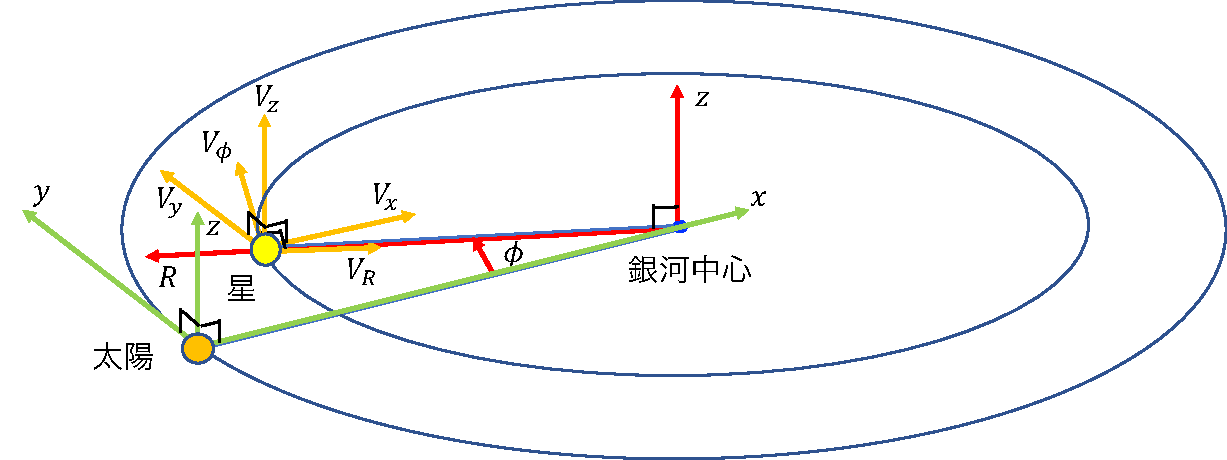
\includegraphics[width=13cm]{fig/Coordinates.pdf}
	\caption{天の川銀河を北銀極方向から斜めに眺め下ろした図。緑線は太陽系を中心とした直交座標系$(x,y,z)$、赤線は銀河系中心を中心とした円筒座標系$(R,\phi,z)$、黄線は直交座標系での星の速度ベクトル$(V_x,V_y,V_z)$を表している。}
	\label{fig:coordinates}
\end{center}
\end{figure*}

さらに軸対称な系では、$C=K=0$となり、
%\footnote[1]{しかしながら、$C$と$K$がゼロであることは銀河系ポテンシャルが軸対称になる上で必要ではないことに注意しなければならない。代わりに太陽が楕円ポテンシャルの主軸の近くに位置する可能性がある。(\cite{KT1994})}
\begin{subequations}
\begin{align}
	A_{\mathrm{sym}} &=\frac{1}{2}\left( \frac{V_{\phi}}{R} - \frac{\partial V_{\phi}}{\partial R} \right)_{R=R_{\odot}} \\
	B_{\mathrm{sym}} &=\frac{1}{2}\left( -\frac{V_{\phi}}{R} - \frac{\partial V_{\phi}}{\partial R} \right)_{R=R_{\odot}}
\end{align} \label{ABsym}
\end{subequations}
はオールトによって実際に得られた式である。$R_{\odot}$は太陽から銀河中心までの距離を表す。軸対称な銀河では、閉じた軌道はほぼ円軌道と近似できるため、このときの軌道の速度$V_{\phi}$は中心力と遠心力のつりあいから$V_{\phi}^2=R \partial\ \Phi/\partial R$を持ち、オールト定数の測定は銀河系ポテンシャル$\Phi$の直接的な制限をすることになる。例えば、調和振動子ポテンシャル$(\Phi \propto R^2)$では、
\begin{align}
\begin{aligned}
    v_{\mathrm{c}} = R \cfrac{\partial \Phi}{\partial R} = 2R^2 \propto R^2 \to v_{\mathrm{c}} \propto R
\end{aligned}
\end{align}
から、
\begin{subequations}
\begin{align}
	A_{\mathrm{sym}} &\propto\frac{1}{2}\left( \frac{R}{R} - \frac{\partial R}{\partial R} \right) = 0\\
	B_{\mathrm{sym}} &\propto \frac{1}{2}\left( -\frac{R}{R} - \frac{\partial R}{\partial R} \right) = 1
\end{align}
\end{subequations}
となる。このとき、銀河回転は剛体回転となり、$B$は銀河の回転周波数と等しくなる。また、回転曲線が平坦なとき$(V_{\phi}=\mathrm{const})$には、定数$a$を用いて$V_{\phi} = a$とすると、
\begin{subequations}
\begin{align}
	A_{\mathrm{sym}} &=\frac{1}{2}\left( \frac{a}{R} - \frac{\partial a}{\partial R} \right) = \frac{1}{2}\frac{a}{R}\\
	B_{\mathrm{sym}} &=\frac{1}{2}\left( -\frac{a}{R} - \frac{\partial a}{\partial R} \right) = -\frac{1}{2}\frac{a}{R}
\end{align}
\end{subequations}
から$A=-B$となる。さらに、全質量が銀河系中心付近に集中してケプラーポテンシャルとなっているとき$(V_{\phi} \propto R^{-1/2})$には、中心力$F$、重力定数$G$、星の質量$M$を用いると、$F = \dfrac{GM}{R^2} = \dfrac{v_{\mathrm{c}}^2}{R}$から
\begin{align}
\begin{aligned}
    v_{\mathrm{c}}^2 = \frac{GM}{R} \to v_{\mathrm{c}} \propto R^{-1/2}
\end{aligned}
\end{align}
となるため、
\begin{subequations}
\begin{align}
	A_{\mathrm{sym}} &\propto \frac{1}{2}\left( \frac{R^{-1/2}}{R} - \frac{\partial R^{-1/2}}{\partial R} \right) = \frac{3}{4}R^{-3/2}\\
	B_{\mathrm{sym}} &\propto \frac{1}{2}\left( -\frac{R^{-1/2}}{R} - \frac{\partial R^{-1/2}}{\partial R} \right) = -\frac{1}{4}R^{-3/2}
\end{align}
\end{subequations}
から$A=-3B$となる。\cite{Oort1927b}は、不定性は大きいものの、視線速度と固有運動から$A\approx 19\,\mathrm{km\,s^{-1} kpc^{-1}}, B\approx -24\,\mathrm{km\,s^{-1} kpc^{-1}}$という値を得た。オールトはこの結果から銀河ポテンシャルは調和振動子ポテンシャルやこれは、まだ天の川銀河が回転していることが定着していなかった頃のことである。このオールトの研究結果は天の川銀河が回転していることの明確な証拠となり、天の川銀河は剛体回転しているというLindbladの提案を棄却した。


%%%%%%%%%%%%%%%%%%%%%%%%%%%%%%%%%%%%%%%%%%%%%%%%%%%%%%%%%%%%%%%%%%%%%%%%
%%%%%%%%%%%%%%%%%%%%%%%%%%%%%%%%%%%%%%%%%%%%%%%%%%%%%%%%%%%%%%%%%%%%%%%%
%%%%%%%%%%%%%%%%%%%%%%%%%%%%%%%%%%%%%%%%%%%%%%%%%%%%%%%%%%%%%%%%%%%%%%%%

\subsection{観測方程式}
ここで、銀河中心を基準とした星の速度を$\delta\pmb{V}$、そして$\delta\pmb{V}$の$x、y$成分を$\delta V_x、\delta V_y$とすると、次のように書ける。
\begin{align}
\begin{aligned}
	\delta\pmb{V} =
	\left(
	\begin{array}{c}
	 	\delta V_x\\
		\delta V_y
	\end{array}
	\right)
	=
	\pmb{H} \cdot \pmb{r}
	=&
	\left(
	\begin{array}{cc}
	 	K+C & A-B\\
		A+B & K-C
	\end{array}
	\right)
	\cdot
	\left(
	\begin{array}{c}
	 	x\\
		y
	\end{array}
	\right)\\
	=&
	\left(
	\begin{array}{c}
	 	(K+C)x + (A-B)y\\
		(A+B)x + (K-C)y
	\end{array}
	\right)
\end{aligned} \label{eq266}
\end{align}

簡単のためにテイラー展開の2次の項$\mathcal{O}(\pmb{r}^2)$は無視している。銀経$l$の位置を太陽に対して速度$(U,V)$で運動している星は視線速度$v_d$、接線速度$v_l$で観測される (図\ref{fig:OD03})。
ある星と太陽との距離を$d$、銀経を$l$とすると、$x = d\cos l,y = d \sin l$と書ける。式(\ref{eq266})を用いると、ある星の視線速度を銀河円盤面 ($b=0^{\circ}$面)に投影した速度$v^*_d$は次の式で表さ
れる。
\begin{align}
\begin{aligned}
	v^*_d &= \frac{1}{d} \pmb{r} \cdot \delta\pmb{V}
	= \frac{1}{d}(x\delta V_x + y\delta V_y) \\
	&= \frac{1}{d} [(K+C)x^2 + (K-C)y^2 + 2Axy] \\
	&= \frac{1}{d} [K(x^2 + y^2) + C(x^2 - y^2) + 2Axy] \\
	&= d(K + C\cos2l + A\sin2l)
\end{aligned} \label{vd}
\end{align}
となる。

式(\ref{vd})から、太陽系近傍の星の視線速度と銀経$l$、距離$d$からオールト定数$A、C、K$を決定することができることがわかる。一方オールト定数$B$は星の固有運動から求めることができる。視線速度に垂直な速度成分である接線速度$v^*_l$は、式(\ref{eq266})を用いて
\begin{align}
\begin{aligned}
	v^*_l &= \frac{1}{d}(\pmb{r} \times \delta\pmb{V})_z = \frac{1}{d}(x\delta V_y - y\delta V_x)\\
	&= \frac{1}{d}[B(x^2 + y^2) + A(x^2 - y^2) - 2Cxy] \\
	&= d(B + A\cos2l - C \sin2l)
\end{aligned}
\end{align}
となる。銀緯$b=0$面の星を見ているとき、太陽系の視線速度成分、接線速度成分を$v_{\odot,d}、v_{\odot,l}$と書くと、
\begin{align}
\begin{aligned}
	\left(
	\begin{array}{c}
	 	v_{\odot,d}\\
		v_{\odot,l}\\
	\end{array}
	\right)
	&=
	\left(
	\begin{array}{cc}
	 	\cos l & \sin l\\
		-\sin l & \cos l\\
	\end{array}
	\right)
	\left(
	\begin{array}{c}
	 	U_{\odot}\\
		V_{\odot}\\
	\end{array}
	\right) \\
	&=
	\left(
	\begin{array}{c}
	 	U_{\odot} \cos l + V_{\odot} \sin l\\
		-U_{\odot} \sin l + V_{\odot} \cos l\\
	\end{array}
	\right)
\end{aligned}
\end{align}
となるから、太陽系から見た視線速度と接線速度$v_d、v_l$は
\begin{subequations}
\begin{align}
    v_d &= v^*_d - v_{\odot,d} =  d(K+A\sin{2l}+C\cos{2l}) -V_{\odot}\sin{l} - U_{\odot}\cos{l} \label{eq:6} \\
    v_l &= v^*_l - v_{\odot,l} = d(B-C\sin{2l}+A\cos{2l}) + U_{\odot}\sin{l} - V_{\odot}\cos{l} \label{eq:7}
\end{align}
\end{subequations}
と表される。


実際には天の川銀河は円盤面上に全ての星が存在するような2次元の構造ではなく、星が円盤面から離れたところにも存在する3次元であるため、$v_d,v_l$の式を直接的には使えない。したがって、銀河円盤面の外の星を一般化するために以下の式を使う。
\begin{subequations}
\begin{align}
	\varpi &= d^{-1} \cos b \\
	v_{\mathrm{los}} &= v_d \cos b + v_z \sin b\\
	\mu^*_l &= \varpi v_l \\
	\mu_b &= \varpi(v_z \cos b - v_d \sin b)
\end{align} \label{OD03}
\end{subequations}
ここで、$\mu^*_l \equiv \mu_l \cos b$ (観測で直接得られる値)である。上式の表記については図(\ref{fig:OD03})を参照されたい。
\begin{figure*}[htbp]
\begin{center}
	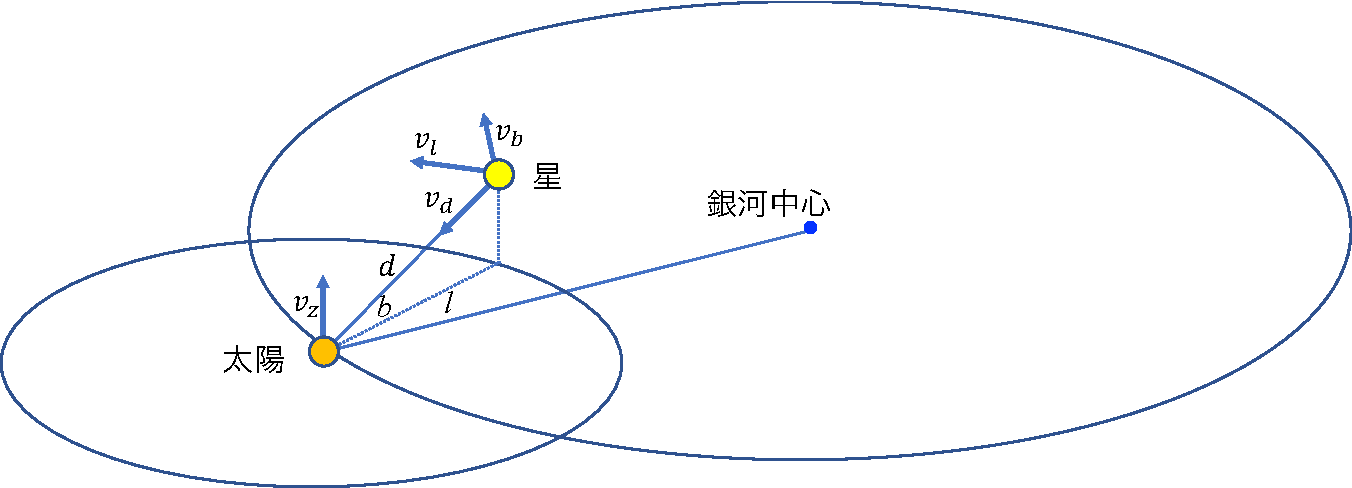
\includegraphics[width=10cm]{fig/figOD2003.pdf}
	\caption{式(\ref{OD03})、式(\ref{Q})で使われている各パラメータが示す量。$l、b$はそれぞれ銀経、銀緯。$a$は星の銀河円盤面での位置と銀河中心、太陽の位置とを結んだときの角度。$d$は星と太陽との距離。$v_l,v_b,v_{\mathrm{los}}$はそれぞれ星の銀経方向、銀緯方向、視線方向の速度。実際の観測量は3次元の速度を持っているため、2次元モデルを使うことができるように円盤から離れた星の位置・速度を円盤面に投影する。}
	\label{fig:OD03}
\end{center}
\end{figure*}
$\mu^*_l$を$\mu^{*,\mathrm{OL}}_l(l_i,b_i,\varpi_i)$、$\mu_b$を$\mu^{\mathrm{OL}}_b$、$v_{\mathrm{los}}$を$v^{\mathrm{OL}}_{\mathrm{los}}$と書くことにすると、
\begin{subequations}
\begin{align}
	\mu^{*,\mathrm{OL}}_l(l_i,b_i,\varpi_i) &= (A\cos2l_i - C\sin2l_i + B)\cos b_i + \varpi_i(U_{\odot}\sin l_i - V_{\odot}\cos l_i) \\
	\mu^{\mathrm{OL}}_b(l_i,b_i,\varpi_i) &= -(A\sin2l_i + C\cos2l_i + K)\sin b_i \cos b_i \nonumber \\
	                          & \hspace{2cm} + \varpi_i[(U_{\odot}\cos l_i + V_{\odot} \sin l_i)\sin b_i - W_{\odot} \cos b_i] \\
	v^{\mathrm{OL}}_{\mathrm{los}}(l_i,b_i,\varpi_i) &= (K + C\cos2l_i + A\sin2l_i)\varpi_i^{-1}  \cos^2 b_i \nonumber\\
	                      & \hspace{2cm} - [(U_{\odot}\cos l_i + V_{\odot} \sin l_i)\cos b_i + W_{\odot} \sin b_i]
\end{align} \label{ObsEq}
\end{subequations}
となり、これが基本的な観測方程式となる。ここで、OLの添字はOort-Lindbladモデルの式であることを示す。また、添字$i$は星ごとの観測量であることを示す。

実際に解析する際の観測方程式の使用方法について簡単に説明する。例えば観測データの中の$i$番目の星が銀経$l_i$、銀緯$b_i$、年周視差$\varpi_i$、固有運動$\mu_ {l,i}$とその誤差$e_{\mu_ {l,i}}$を持っているとき、$\mu_{l,i}$が標準偏差$e_{\mu_ {l,i}}$の正規分布の確率分布で$l_i、b_i、\varpi_i$の関数で書ける$\mu^{*,\mathrm{OL}}_l(l_i,b_i,\varpi_i)$と一致すると仮定する。これにより、式(\ref{ObsEq})の中の$\mu^{*,\mathrm{OL}}_l(l_i,b_i,\varpi_i)$の式に含まれているパラメータ$A、B、C、U_{\odot}、V_{\odot}$が得られることになる。同様に$\mu_{b,i}$と$\mu^{\mathrm{OL}}_b(l_i,b_i,\varpi_i)$とでフィッティングをすることでパラメータ$A、C、K、U_{\odot}、V_{\odot}、W_{\odot}$が得られ、$v^{\mathrm{OL}}_{\mathrm{los}}(l_i,b_i,\varpi_i)$も同様にパラメータを得られる。先行研究では固有運動の式2つのみでフィッティングをしているものもあるが、可能な限り正確にパラメータ推定を行うためには式1つや2つよりも式3つで行う方が良いため、本論文では3つの式を用いて解析している。

%%%%%%%%%%%%%%%%%%%%%%%%%%%%%%%%%%%%%%%%%%%%%%%%%%%%%%%%%%%%%%%%%%%%%%%%
%%%%%%%%%%%%%%%%%%%%%%%%%%%%%%%%%%%%%%%%%%%%%%%%%%%%%%%%%%%%%%%%%%%%%%%%
%%%%%%%%%%%%%%%%%%%%%%%%%%%%%%%%%%%%%%%%%%%%%%%%%%%%%%%%%%%%%%%%%%%%%%%%

\section{速度分散を考慮した場合への拡張} % Olling & Dehnenを参考に書く
前節では力学的に冷たい系、すなわち速度分散が小さく無視できる系を仮定したが、実際の銀河系円盤の星は無視できない程度の速度分散を持っている。本節では、従来のOort-Lindbladモデルによる観測方程式を速度分散を考慮した場合へ拡張することを考える。

\subsection{従来のOort-Lindbladモデルの問題点} % ここにYu & Liu の年齢速度分散関係の図も載せるとよい。
従来のOort-Lindbladモデルは速度分散が非常に小さく、系統速度に比べて無視できるような系を仮定したモデルである。しかし、現実の銀河円盤星は無視できない大きさの速度分散を持っていることが知られており、従来のモデルをそのまま用いると測定がうまくいかない可能性がある。

図\cite{YL18}によって調べられた年齢-速度分散関係である。彼らはLarge Sky Area Multi-Object Fiber Spectroscopic Telescope (LAMOST)とTycho-Gaia Astrometric Solution (TGAS; \cite{Gaia2016}) をクロスマッチさせて、3564個の準巨星分枝星/赤色巨星分枝星に対して年齢推定を行った。金属量が少ない$([\mathrm{Fe}/\mathrm{H}] < 0.2\,\mathrm{dex})$星、金属量が多い$([\mathrm{Fe}/\mathrm{H}] < 0.2\,\mathrm{dex})$星と全金属量の星に関してそれぞれ年齢-速度分散関係を求めている。図\ref{VDbyYL18}を見ると、年齢と速度分散との間に明確な依存性が見られる。

\begin{figure*}[htbp]
\begin{center}
	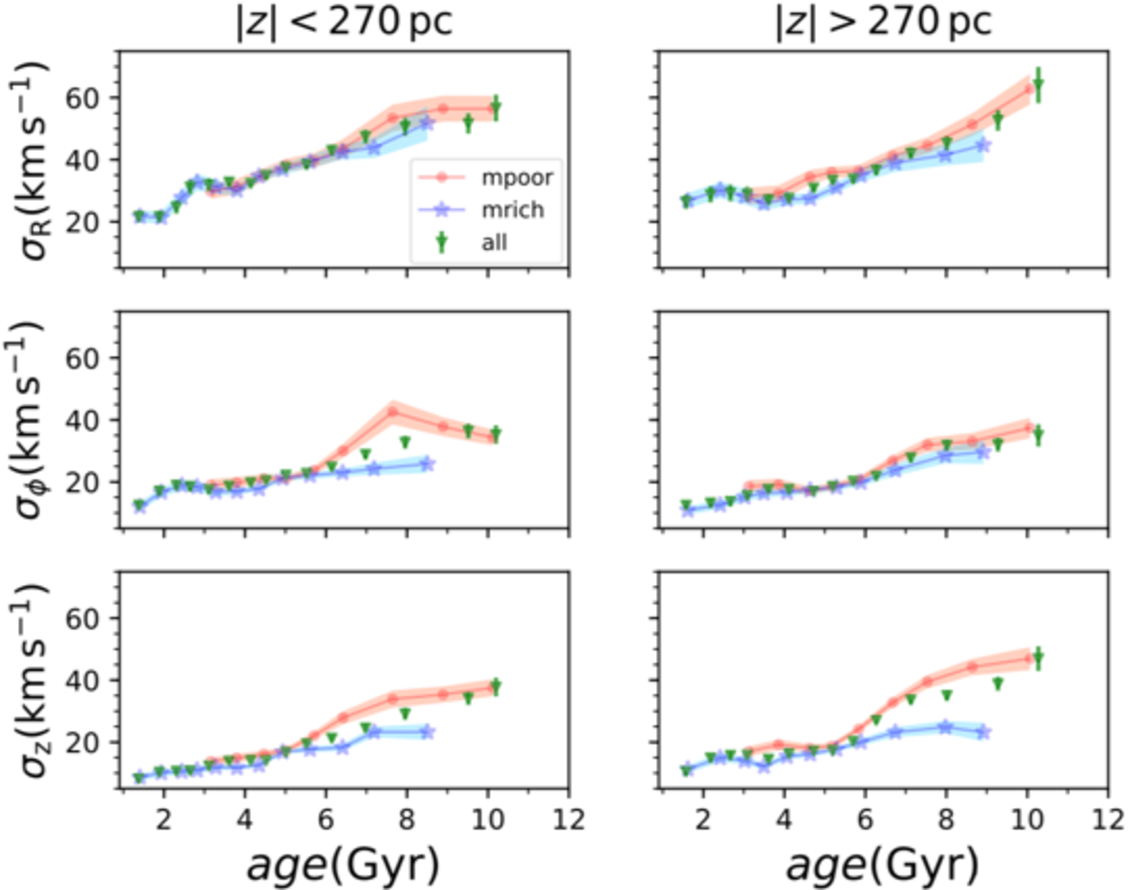
\includegraphics[width=12cm]{fig/YuLiu18_VD.pdf}
	\caption{太陽近傍星の年齢・速度分散関係\cite{YL18}。$\sigma_R、\sigma_{\phi}、\sigma_z$は円筒座標系$(R,\phi,z)$での速度分散。円盤面からの距離$|z|<270\,\mathrm{pc}$と$|z|>270\,\mathrm{pc}$とで区切っている。色の違いは金属量の違いを表しており、ピンク色は金属量が少ない (metal poor) サンプル、青色は金属量が多い (metal rich) サンプル、緑色の点は両方を合わせたサンプルの速度分散となっている。}
	\label{VDbyYL18}
\end{center}
\end{figure*}

%%%%%%%%%%%%%%%%%%%%%%%%%%%%%%%%%%%%%%%%%%%%%%%%%%%%%%%%%%%%%%%%%%%%%

大量な星のサンプルの固有運動と視線速度からオールト定数を決定するとき、それらの値を出すときの過程と潜在的な平均速度場に関する解釈の両方を含む様々な問題に直面する。

まず、若い星では運動集団や渦状腕のような非平衡な効果が平均速度$\overline{\pmb{v}}$に影響する。これは主に小さい速度分散の集団に影響する。また、サンプル数が少なすぎる場合、系統速度場の中の太陽近傍の変則的なものがオールト定数に影響する。さらに、特に古い星ではasymmetric driftの効果によって円運動の系統速度から大きく外れる。軸対称な系では、この効果はStr\"{o}mbergのasymmetric drift関係を用いて推定できる。この効果により、$A$は$3\,\mathrm{km\,s^{-1}kpc}$に満たない程度の値だけ小さくなるが、$B$はほとんど変化しない。

太陽から遠いサンプルを使用するほど、系統速度のテイラー展開の高次の項が効いてきてしまう。年周視差と速度の間に非線形の相関がある場合にこの項は特に大きく影響する。銀河系のバーのOLR (outer Lindblad resonance) が効く場所では不連続な系統場が発生し、それがオールト定数の測定を間違えさせる。年周視差の平均$\overline{\varpi}$がサンプルの銀経$l$の方向に対して依存性 (モード) を持ってしまう状態をモードミキシング (Mode mixing) という。モードミキシングがあると、固有運動は数$\mathrm{km\,s^{-1}kpc}$までの範囲でオールト定数と区別できなくなってしまう。本論文で使用する観測データのモードについては\ref{観測データ}で記述する。

%表\ref{table1}では、\cite{OD03}を参考にオールト定数を決定するときの問題点を挙げている。

% \begin{table}[htb]
% \centering
% {\small
%   \begin{tabular}{c|c|p{10cm}} \hline
%     状態 & 表記法 & 定義と説明\\ \hline
%     1 & $A,B,C,K$ & オールト定数:銀河ポテンシャル中の閉じた軌道で作られる(仮定の)速度場$\pmb{v}(\pmb{r})$の発散、回転、剪断\\
%     2$^a$ & $\overline{A},\overline{B},\overline{C},\overline{K}$ & 最も得たい値:星の集団の速度場$\pmb{v}(\pmb{r})$の発散、回転、剪断\\
%     3$^b$ & $\widetilde{A},\widetilde{B},\widetilde{C},\widetilde{K}$ & 実際に得られる値:星の集団から測定される固有運動のフーリエ係数\\
%     \hline
%   \end{tabular} \label{table1}
% \vskip 3pt
% \begin{minipage}{13cm}
% \textit{$^a$}状態1と2の違いの理由として考えられるものを挙げる。(i)若い星:運動集団や渦状腕のような非平衡の効果が閉じた軌道の速度場から$\pmb{\overline{v}}$を予想外な値に導く。これは主に小さい速度分散の集団に影響する。(ii)サンプルの大きさが小さすぎる場合、系統場(streaming field)の中の太陽近傍の変則的なものがオールト定数に反映される。(iii)特に古い星ではasymmetric driftの効果によって閉じた軌道の系統速度から外れる。軸対称な系では、この効果はStr\"{o}mbergのasymmetric drift関係を用いて推定できる。この効果により、$A$は$3\,\mathrm{km\,s^{-1}kpc}$に満たない程度の値だけ小さくなるが、$B$はほとんど変化しない。\\
% \textit{$^b$}状態2と3の違いの理由として考えられるものを挙げる。(i)太陽から遠いサンプルを使用するほど、系統速度のテイラー展開の高次の項が効いてきてしまう。年周視差と速度の間に非線形の相関がある場合にこの項は特に大きく影響する。(ii)銀河系のバーのOLR (outer Lindblad resonance) が効く場所では不連続な系統場が発生し、それがオールト定数の測定を間違えさせる。(iii)年周視差の平均$\overline{\varpi}$がサンプルの銀経$l$の方向に対して依存性 (モード) を持ってしまう状態をモードミキシング (Mode mixing) という。モードミキシングがあると、固有運動は数$\mathrm{km\,s^{-1}kpc}$までの範囲でオールト定数と区別できなくなってしまう。
% \end{minipage}
% }
% \end{table}



%%%%%%%%%%%%%%%%%%%%%%%%%%%%%%%%%%%%%%%%%%%%%%%%%%%%%%%%%%
%%%%%%%%%%%%%%%%%%%%%%%%%%%%%%%%%%%%%%%%%%%%%%%%%%%%%%%%%%
%%%%%%%%%%%%%%%%%%%%%%%%%%%%%%%%%%%%%%%%%%%%%%%%%%%%%%%%%%


\subsection{asymmetric drift \label{sec_AD}} % 導出&物理的解釈を書く
asymmetric drift速度$\pmb{v}_{\mathrm{a}}$は、天体が銀河系円盤を閉じた軌道で回転するときの速度$\pmb{v}$と系統速度$\overline{\pmb{v}}$を用いて次のように表される。
\begin{align}
\begin{aligned}
    \pmb{v}_{\mathrm{a}} \equiv \pmb{v}- \overline{\pmb{v}}\\
\end{aligned} \label{AD}
\end{align}
ここで、$\pmb{v}_{\mathrm{a}}$はasymmetric drift速度である。この速度は、太陽近傍における系統速度$\overline{\pmb{v}}$の速度$\pmb{v}$からの遅れを表す。この区別を明確にするために、式(\ref{AD})のようにオールト定数を書くと、以下のように書ける。
\begin{subequations}
\begin{align}
	\overline{A} &= A - A_{\mathrm{a}} \\
	\overline{B} &= B - B_{\mathrm{a}} \\
	\overline{C} &= C - C_{\mathrm{a}} \\
	\overline{K} &= K - K_{\mathrm{a}}
\end{align}
\end{subequations}
近傍の系統運動との相対的な太陽運動はLSR (Local Standard of Rest)に対しての太陽運動とasymmetric driftとに分解される(図\ref{fig1})。

\begin{figure*}[htbp]
\begin{center}
	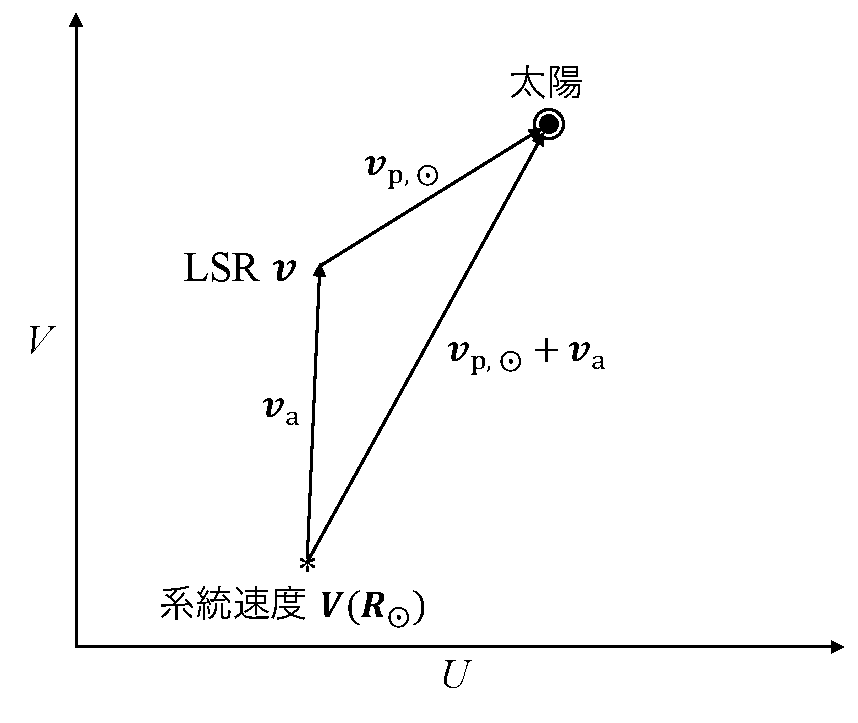
\includegraphics[width=10cm]{fig/various_velocities.pdf}
	\caption{太陽運動とasymmetric driftのスケッチ。$U、V$はそれぞれ太陽を原点として銀河中心方向、円軌道の回転方向の速度。サンプル星の系統速度$\pmb{\overline{v}}$は速度$\pmb{v}$のLSRからasymmetric drift\,$\pmb{v}_{\mathrm{a}}$の分遅れる。太陽の特異運動$\pmb{v}_{\odot}$は観測された系統速度$\pmb{\overline{v}}$に対する太陽の速度を得るために$\pmb{v}_{\mathrm{a}}$を足す必要がある。}
	\label{fig1}
\end{center}
\end{figure*}

力学平衡状態でかつ軸対称な銀河では、$\pmb{v}_{\mathrm{a}}$のうち方位角成分$v_{\mathrm{a}}$のみが存在し、ランダムな運動 (特異運動) は系統運動に比べて非常に小さく、これはStr\"{o}mbergの関係(Jeans方程式からの導出は付録\ref{sec_JeansEq}を参照)から近似される。付録の式(\ref{Jeans_Cylindrical_pr})をここでも書く。
\begin{align}
	\frac{\partial (\nu \overline{V_R^2})}{\partial R} + \frac{\partial (\nu \overline{V_R v_z})}{\partial R} + \nu\left(\frac{\overline{V_R^2} - \overline{V_{\phi}^2}}{R} + \frac{\partial \Phi}{\partial R} \right) = 0 \label{eqJeans448}
\end{align}
この式は円筒座標系で表示されたJeans方程式において動径方向の運動量$p_R$の1次モーメントを取ることで得られる。式(\ref{eqJeans448})の第2項は無視できるものとし、$\overline{V_R}=0$とすると、
\begin{align}
	\frac{\overline{V_{\phi}^2}}{R} = \frac{1}{\nu}\frac{\partial(\nu\sigma_R^2)}{\partial R} + \frac{\partial \Phi}{\partial R} \label{eqJeans452}
\end{align}
となる。また、円運動する星の速度を$v_{\mathrm{c}}$と書くと、中心力と遠心力とのつり合いより$\frac{v_{\mathrm{c}}^2}{R}=\frac{\partial \Phi}{\partial R}$と書ける。この式と式(\ref{eqJeans452})とを比較すると、$\frac{1}{\nu}\frac{\partial(\nu\sigma_R^2)}{\partial R}$は天の川銀河円盤内では負の値を持つことから、$\overline{V_{\phi}^2}$は$v_{\mathrm{c}}^2$に比べて$\frac{1}{\nu}\frac{\partial(\nu\sigma_R^2)}{\partial R}$の分だけ遅くなることが分かる。式(\ref{eqJeans448})を変形し、式(\ref{AD})を使用すると
\begin{align}
\begin{aligned}
    v_{\mathrm{a}} \simeq \frac{\overline{V_R^2}}{2V_{\phi}} \left[\frac{\sigma_{\phi}^2}{\overline{V_R^2}} - 1 - \frac{\partial \ln(\nu \overline{V_R^2})}{\partial \ln R} - \frac{R}{\overline{V_R^2}}\frac{\partial \overline{V_R v_z}}{\partial z}\right] \\
    = \frac{\sigma_R^2}{2V_{\phi}} \left[\frac{\sigma_{\phi}^2}{\sigma_R^2} - 1 - \frac{\partial \ln(\nu \sigma_R^2)}{\partial \ln R} - \frac{R}{\sigma_R^2}\frac{\partial \sigma_{Rz}^2}{\partial z}\right]
\end{aligned} \label{AD2}
\end{align}
という式が得られる。ここで、$\nu$は星密度、$\sigma_{ij}^2 \equiv \overline{(v_i-\overline{v_i})(v_j-\overline{v_j})}=\overline{v_i v_j}-\overline{v_i}\ \overline{v_j}$は速度分散テンソルを示し、ここでは広く使われるように$\sigma_{ii}^2$を$\sigma_i^2$と短く書いている。$i,j$はそれぞれ座標系の異なる向きである。式(\ref{AD2})の1行目から2行目への式変形では$\overline{V_R}=0$と仮定している。式(\ref{AD2})から、asymmetric driftは動径速度分散の関数であり、円軌道速度と速度楕円体の軸比、動径速度分散と星密度の傾きにも依存することがわかる。

図\ref{AD_image}は$v_{\mathrm{a}}$の物理的イメージである。式(\ref{eqJeans452})の$\frac{\overline{V_{\phi}^2}}{R}$は遠心力、$\frac{1}{\nu}\frac{\partial(\nu\sigma_R^2)}{\partial R}$は速度分散勾配による圧力、$\frac{\partial \Phi}{\partial R}$は重力による中心力にあたる。$\frac{1}{\nu}\frac{\partial(\nu\sigma_R^2)}{\partial R}$が天の川銀河の内側から外側に向かって圧力のように働き、銀河回転速度を遅くする。
\begin{figure*}[htbp]
\begin{center}
	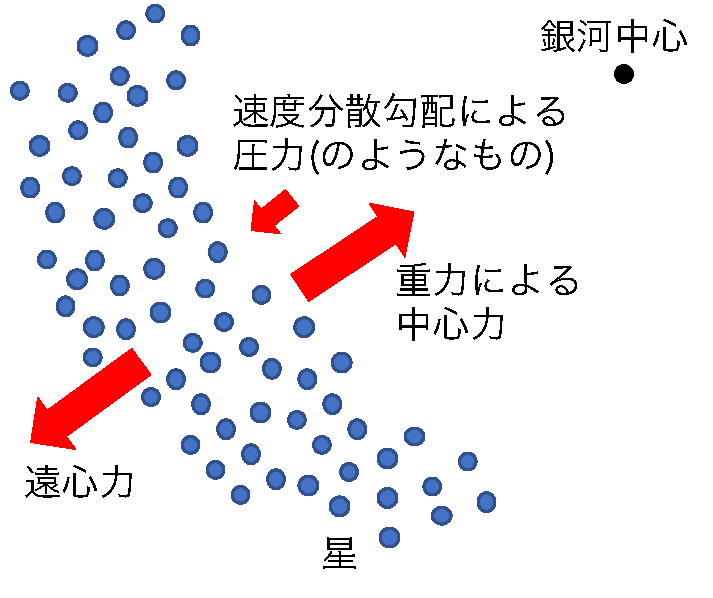
\includegraphics[width=7cm]{fig/AD_image.pdf}
	\caption{asymmetric driftの物理的イメージ。速度分散勾配が圧力のように働く。}
	\label{AD_image}
\end{center}
\end{figure*}

ここで、速度楕円体の説明をする。空間上のある$i$方向の速度分散は$\sigma_i^2 \equiv \overline{(v_i-\overline{v_i})}^2$、$i$方向と$j$方向の間の速度分散テンソルは$\sigma_{ij}^2 \equiv \overline{(v_i-\overline{v_i})(v_j-\overline{v_j})}$と定義される。このとき、$\sigma_i$を半長軸とする楕円体を定義でき、これを速度楕円体と呼ぶ。図\ref{fig:ve}は速度楕円体を2次元面に投影したときの例である。速度楕円体は一般に3軸非対称であり、半長軸の方向は座標軸とは一致するとは限らない。速度楕円体の長軸と座標軸との傾き、例えば$i$軸から$j$軸に向かって$l_{ij}$だけ傾いているとき、
\begin{align}
    \tan(2l_{ij}) = \frac{2\sigma _{ij}^2}{\sigma_i^2 \sigma_j^2}
\end{align}
と表すことができる。

\begin{figure*}[htbp]
\begin{center}
	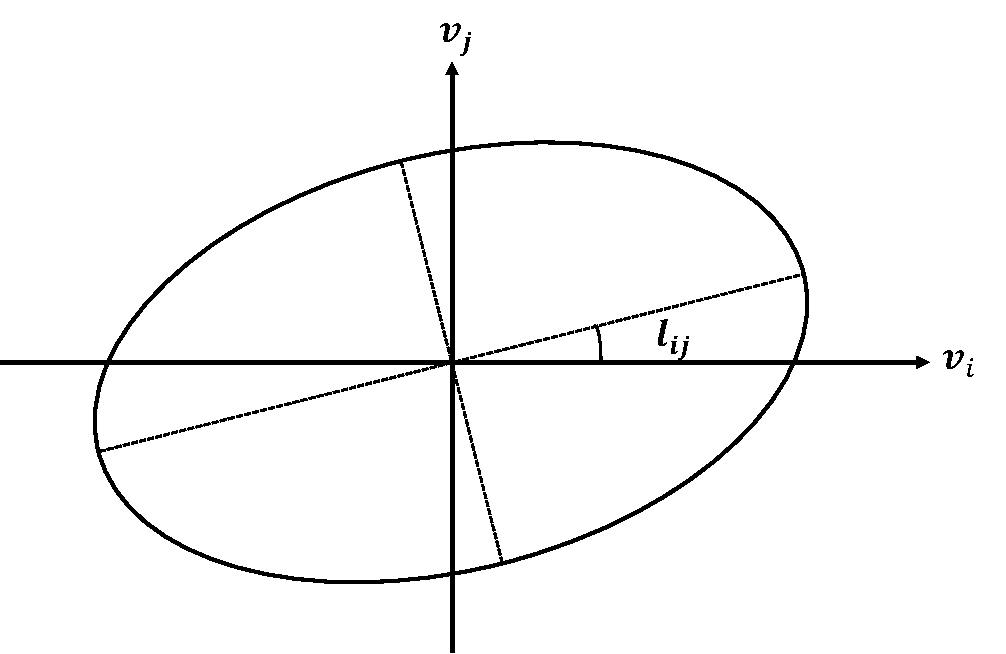
\includegraphics[width=10cm]{fig/velocity_ellipsoid.pdf}
	\caption{速度楕円体を2次元に投影したときの図。楕円は速度分散の1$\sigma$にあたる点を結んだ線である。$l_{ij}$は座標軸を図のようにとったときの楕円の主軸との傾きを表す。}
	\label{fig:ve}
\end{center}
\end{figure*}

式(\ref{AD2})について、\cite{BT2008}の近似にしたがって式変形をしてみる。$\sigma_{\phi}^2/\sigma_R^2 = 0.35$とする。$\nu、\sigma_R^2 \propto e^{-R/h_R}、R/h_R = 3.2$とするとき、
$\frac{\sigma_{\phi}^2}{\sigma_R^2} - 1 - \frac{\partial \ln{(\nu \sigma_R)}}{\partial \ln{R}} = 0.35 - 1 + 6.4 = 5.75$となる。式(\ref{AD2})の右辺最終項について、\cite{BT2008}では次の2つの場合について書かれている。
(i)速度楕円体の主軸が$(R,\phi,z)$の座標軸に沿っているときには$\frac{\partial(\overline{V_R v_z})}{\partial z} = 0$となる。
(ii)速度楕円体の主軸が銀河中心を中心とした球対称座標系$(r,\theta,\phi)$に沿っているとき、$\overline{V_R v_z} \simeq (\sigma_R^2 - \sigma_{\sigma}^2)\frac{z}{R}$から$\frac{R}{\sigma_R^2} \frac{\partial (\overline{V_R v_z})}{\partial z} \simeq 0.8$となる。$\frac{\partial(\overline{V_R v_z})}{\partial z}$は(i)、(ii)の中間的な値であるとすると、式(\ref{AD2})の角括弧内は$5.4 \pm 0.4$と計算できる。さらに回転速度$V_{\phi} = \SI{200}{km.s^{-1}}$とすると、$v_{\mathrm{a}} \simeq \frac{\sigma_R^2}{82 \pm 6\,\si{km.s^{-1}}}$となる。この式をさらにシンプルに表現すると
\begin{align}
\begin{aligned}
    v_{\mathrm{a}} \simeq \frac{\sigma_R^2}{80}
\end{aligned} \label{AD3}
\end{align}
となる (\cite{BT2008})。



%%%%%%%%%%%%%%%%%%%%%%%%%%%%%%%%%%%%%%%%%%%%%%%%%%%%%%%%%%%%%%%%%%%%%%%%%%%%%%%%%%%%%%%%
%%%%%%%%%%%%%%%%%%%%%%%%%%%%%%%%%%%%%%%%%%%%%%%%%%%%%%%%%%%%%%%%%%%%%%%%%%%%%%%%%%%%%%%%

\subsection{asymmetric driftのオールト定数への影響}
$A,B,C,K$は (仮定の) 閉じた軌道の系統場から出され、ポテンシャルに従った項で直接的に解釈される一方、$\overline{A},\overline{B},\overline{C},\overline{K}$は実際の星の集団の系統場を表す。$\overline{A},\overline{B},\overline{C},\overline{K}$は式(\ref{eq2})あるいは(\ref{eq2.5a})-(\ref{eq2.5d})において$\pmb{v}$を$\pmb{\overline{v}}$で置き換えたもので、$A_{\mathrm{a}},B_{\mathrm{a}},C_{\mathrm{a}},K_{\mathrm{a}}$は同じく$\pmb{v}$を$\pmb{v}_{\mathrm{a}}$で置き換えたものである。

ここで、式(\ref{AD2})について、$\nu,\sigma_{ij}$がそれぞれスケール長$h_R,h_{\sigma}$で指数関数的に変化すると仮定し、$\nu \propto e^{
-R/h_R}、\sigma_{ij}^2 \propto e^{-R/h_{\sigma}}、hv_{\mathrm{a}} \simeq \sigma_{R}^2$という仮定を用いる。また、右辺第3項は$-\partial \mathrm{ln}(\nu \sigma_R^2)/\partial \mathrm{ln} R = R(1/h_R + 1/h_{\sigma})$と変形できる。さらに右辺第4項は無視できるから、
\begin{align}
\begin{aligned}
    2V_{\phi}v_{\mathrm{a}} \simeq \sigma_R^2 \left[\frac{\sigma_{\phi}^2}{\sigma_R^2} - 1 + R\left(\frac{1}{h_R} + \frac{2}{h_{\sigma}}\right)\right]
\end{aligned} \label{AD5}
\end{align}
となる。ここで、$\sigma_{ij} \propto e^{-R/h_{\sigma}}$から、$D$を定数として$\sigma_{\phi}^2/\sigma_R^2 - 1 = D$と書けるから、
\begin{align}
\begin{aligned}
    2V_{\phi}v_{\mathrm{a}} \simeq \sigma_R^2 \left[D + R\left(\frac{1}{h_R} + \frac{2}{h_{\sigma}}\right)\right]
\end{aligned} \label{AD6}
\end{align}
式 (\ref{AD6})の両辺のlogをとり$R$で微分すると、
\begin{align}
\begin{aligned}
    \ln2+\ln V_{\phi}+\ln v_{\mathrm{a}} &\simeq \ln \sigma_R^2 +\ln \left[D + R\left(\frac{1}{h_R} + \frac{2}{h_{\sigma}}\right)\right] \\
    \frac{\partial \ln V_{\phi}}{\partial R}+\frac{\partial \ln v_{\mathrm{a}}}{\partial R} &\simeq -\frac{2}{h_{\sigma}} + \frac{1/h_R + 1/h_{\sigma}}{D +R\left(1/h_R + 1/h_{\sigma}\right)} \\
\end{aligned} \label{AD8}
\end{align}
したがって、式(\ref{AD6}),(\ref{AD8})と$hv_{\mathrm{a}} \simeq \sigma_R^2$から
\begin{align}
\begin{aligned}
    \frac{\partial \mathrm{ln}v_{\mathrm{a}}}{\partial R} \simeq -\frac{2}{h_{\sigma}} + \frac{h}{2V_{\phi}}\left(\frac{1}{h_R} + \frac{2}{h_{\sigma}}\right) - \frac{\partial \mathrm{ln}V_{\phi}}{\partial R}
\end{aligned} \label{AD9}
\end{align}
となる。

asymmetric driftは軸対称を仮定していることから、式(\ref{ABsym}),(\ref{AD9})を利用して$A_{\mathrm{a}},B_{\mathrm{a}}$は次のように表すことができる。
\begin{subequations}
\begin{align}
	A_{\mathrm{a}} &=\frac{1}{2}\left( \frac{v_{\mathrm{a}}}{R} - \frac{\partial v_{\mathrm{a}}}{\partial R} \right)_{R=R_{\odot}} = \frac{v_{\mathrm{a}}}{2}\left[\frac{1}{R_{\odot}} + \frac{2}{h_{\sigma}} - \frac{h}{2V_{\phi}}\left(\frac{1}{h_R} + \frac{2}{h_{\sigma}}\right)\right] \\
	B_{\mathrm{a}} &=\frac{1}{2}\left( -\frac{v_{\mathrm{a}}}{R} - \frac{\partial v_{\mathrm{a}}}{\partial R} \right)_{R=R_{\odot}} = \frac{v_{\mathrm{a}}}{2}\left[-\frac{1}{R_{\odot}} + \frac{2}{h_{\sigma}} - \frac{h}{2V_{\phi}}\left(\frac{1}{h_R} + \frac{2}{h_{\sigma}}\right)\right]
\end{align} \label{ABaxisym}
\end{subequations}
$R_{\odot}=8.2\,\mathrm{km\,s^{-1}},h_R =2.68\,\mathrm{kpc}, h_{\sigma}=9\,\mathrm{kpc}$ (\cite{Piffl14}),$V_{\phi}=236\,\mathrm{km\,s^{-1}}$ (\cite{Kawata2019}) とするとき
$A_{\mathrm{a}}\approx0.122v_{\mathrm{a}}, B_{\mathrm{a}}\approx0.003v_{\mathrm{a}}$となり、$h_R,R_{\odot},V_{\phi}$とはほぼ独立している。すなわち、$B$はasymmetric driftの影響をほとんど受けないが、$A_{\mathrm{a}}$は$v_{\mathrm{a}}=20$のときには2.4程度の大きさとなり、asymmetric driftの影響を少し受ける。

%%%%%%%%%%%%%%%%%%%%%%%%%%%%%%%%%%%%%%%%%%%%%%%%%%%%%%%%%%%%%%%%%%%%%%%%%%%%%%%%%%%%%%%%
%%%%%%%%%%%%%%%%%%%%%%%%%%%%%%%%%%%%%%%%%%%%%%%%%%%%%%%%%%%%%%%%%%%%%%%%%%%%%%%%%%%%%%%%

\subsection{asymmetric driftを考慮した観測方程式 \label{sec_ObsAD}}
ここで、観測方程式にasymmetric drift項を追加することを考える。円筒座標系で$(0,v_a,0)$とする。また、$\bf{P、Q}$はそれぞれ$(V_x,V_y,v_z) \to (v_l,v_ b,v_{\mathrm{los}})、(v_{R},V_{\phi},v_z) \to (V_x,v_ y,v_z)$のようにベクトルを変換する行列であるとする。このとき$\bf{P,Q}$は
\begin{align}
\begin{aligned}
	\bf{P}=
	\left(
	\begin{array}{ccc}
	 	-\sin{l} & -\cos{l}\sin{b} & \cos{l}\cos{b}\\
		 \cos{l} &  \sin{l}\cos{b} & \sin{l}\cos{b}\\
		0 & \cos{b} & \sin{b}
	\end{array}
	\right)
\end{aligned}
\end{align}
\begin{align}
\begin{aligned}
	\bf{Q}=
	\left(
	\begin{array}{ccc}
	 	\cos{\phi} & -\sin{\phi} & 0\\
		\sin{\phi} &  \cos{\phi} & 0\\
		0 & 0 & 1
	\end{array}
	\right)
\end{aligned} \label{Q}
\end{align}
ここで、角度$a$は図\ref{fig:a}のようにとっている。
\begin{figure*}[htbp]
\begin{center}
	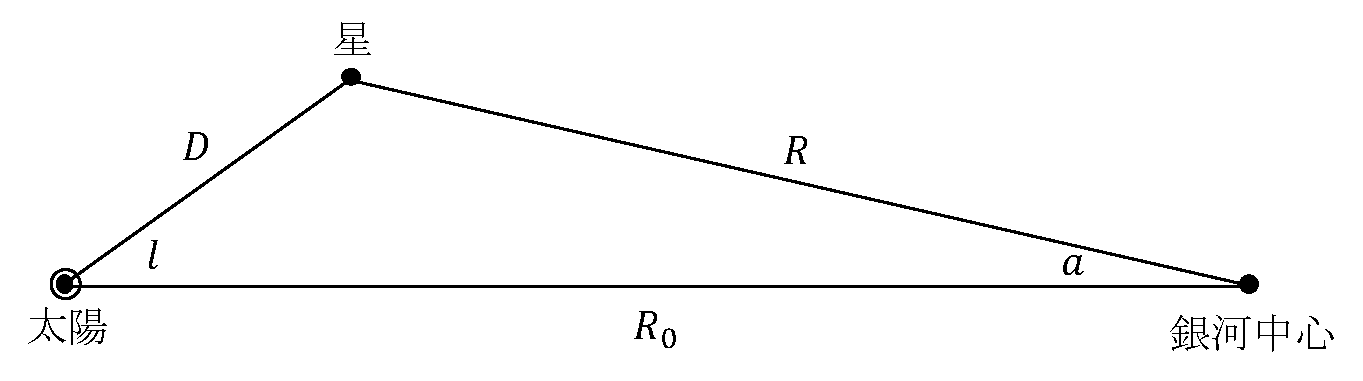
\includegraphics[width=10cm]{fig/coordinate_a.pdf}
	\caption{角度$a$と他のパラメータのとり方}
	\label{fig:a}
\end{center}
\end{figure*}
銀河座標系でのasymmetric drift項を$(v_{\mathrm{a},l},v_{\mathrm{a},b},v_{\mathrm{a},\gamma})$と書くと、
\begin{align}
\begin{aligned}
	\left(
	\begin{array}{c}
	 	v_{a,l}\\
		v_{a,b}\\
		v_{a,\mathrm{los}}
	\end{array}
	\right)
	=& \bf{P} \bf{Q}
	\left(
	\begin{array}{c}
	 	0\\
		v_a\\
		0
	\end{array}
	\right)
\end{aligned}
\end{align}
となる。式(\ref{ObsEq})にasymmetric drift項を追加した式は
\begin{subequations}
\begin{align}
	\mu^{*,\mathrm{AD}}_l(l_i,b_i,\varpi_i) &= (A\cos2l_i - C\sin2l_i + B)\cos b_i + \varpi_i(U_{\odot}\sin l_i - V_{\odot}\cos l_i) - \varpi_i v_{a,l} \\
	\mu^{\mathrm{AD}}_b(l_i,b_i,\varpi_i) &= -(A\sin2l_i + C\cos2l_i + K)\sin b_i \cos b_i \nonumber \\
	                          & \hspace{2cm} + \varpi_i[(U_{\odot}\cos l_i + V_{\odot} \sin l_i)\sin b_i - W_{\odot} \cos b_i] - \varpi_i v_{a,b} \\
	v^{\mathrm{AD}}_{\mathrm{los}}(l_i,b_i,\varpi_i) &= (K + C\cos2l_i + A\sin2l_i)\varpi_i^{-1} cos^2 b_i \nonumber \\
	                      & \hspace{2cm} - [(U_{\odot}\cos l_i + V_{\odot} \sin l_i)\cos b_i + W_{\odot} \sin b_i] - v_{a,\gamma}
\end{align} \label{ObsEqAD}
\end{subequations}
となる。添字のADは、asymmetric driftを考慮したモデルの式であることを示している。



%%%%%%%%%%%%%%%%%%%%%%%%%%%%%%%%%%%%%%%%%%%%%%%%%%%%%%%%%%%%%%%%%%%%%%%%
%%%%%%%%%%%%%%%%%%%%%%%%%%%%%%%%%%%%%%%%%%%%%%%%%%%%%%%%%%%%%%%%%%%%%%%%
%%%%%%%%%%%%%%%%%%%%%%%%%%%%%%%%%%%%%%%%%%%%%%%%%%%%%%%%%%%%%%%%%%%%%%%%



% \section{Asymmetric drift \label{Asymmetric drift}}
% この節では\cite{BT2008}にしたがってasymmetric driftについて説明する。

% 重力ポテンシャルが$\Phi$のとき$H=\frac{1}{2}v^2 + \Phi(\pmb{x},t)$で書けるような直交座標系での無衝突ボルツマン方程式は次のようになる。
% \begin{align}
% 	\frac{\partial f}{\partial t} + p_R\frac{\partial f}{\partial R} + \frac{p_{\phi}}{R^2}\frac{\partial f}{\partial \phi} + p_z\frac{\partial f}{\partial z} - \left(\frac{\partial \Phi}{\partial R} - \frac{p_{\phi}^2}{R^3} \right)\frac{\partial f}{\partial p_R} - \frac{\partial \Phi}{\partial \phi}\frac{\partial f}{\partial p_{\phi}} - \frac{\partial \Phi}{\partial z}\frac{\partial f}{\partial p_z} = 0
% \end{align}
% 円筒座標系では$H = \frac{1}{2}(p_R^2 + p_{\phi}^2/R^2 + p_z^2) + \Phi$となり、そのため
% \begin{align}
% 	\frac{\partial f}{\partial t} + \frac{\partial f}{\partial \pmb{q}} \frac{\partial H}{\partial \pmb{p}} - \frac{\partial f}{\partial \pmb{p}} \frac{\partial H}{\partial \pmb{q}} = 0
% \end{align}
% から
% \begin{align}
% 	\frac{\partial f}{\partial t} + p_R\frac{\partial f}{\partial R} + \frac{p_{\phi}}{R^2}\frac{\partial f}{\partial \phi} + p_z\frac{\partial f}{\partial z} - \left(\frac{\partial \Phi}{\partial R} - \frac{p_{\phi}^2}{R^3} \right)\frac{\partial f}{\partial p_R} - \frac{\partial \Phi}{\partial \phi}\frac{\partial f}{\partial p_{\phi}} - \frac{\partial \Phi}{\partial z}\frac{\partial f}{\partial p_z} = 0   \label{eq193}
% \end{align}
% のようになる。考えている系が定常状態で軸対称であると仮定すると、$t$と$\phi$に関する微分の項は全て消える。これらの仮定から、式(\ref{eq193})は
% \begin{align}
% 	p_r\frac{\partial f}{\partial R} + p_z\frac{\partial f}{\partial z} - \left(\frac{\partial \Phi}{\partial R} - \frac{p_{\phi}^2}{R^3} \right)\frac{\partial f}{\partial p_R} - \frac{\partial \Phi}{\partial z}\frac{\partial f}{\partial p_z} = 0    \label{eq196}
% \end{align}
% と簡単に書ける。この式に$p_R$をかけて全運動量で積分し、式(\ref{eq196})を用いて
% \begin{align}
% 	\frac{\partial (\nu \overline{v_{\mathrm{los}}^2})}{\partial R} + \frac{\partial (\nu \overline{v_{\mathrm{los}} v_z})}{\partial R} + \nu\left(\frac{\overline{v_{\mathrm{los}}^2} - \overline{V_{\phi}^2}}{R} + \frac{\partial \Phi}{\partial R} \right) = 0   \label{eq200}
% \end{align}
% となる。ここで、asymmetric drift速度
% \begin{align}
% 	v_{\mathrm a} \equiv v_{\mathrm c} - \overline{V_{\phi}}
% \end{align}
% を考える。$v_{\mathrm c}$は太陽近傍での円軌道速度である。

% 今、円盤は定常状態でその赤道面に対して対称であると考える。また、太陽は銀河赤道の近くに位置しているため、$z=0$での式(\ref{eq200})を考えればよい。対称性より$\partial \nu/\partial z = 0$であるから、次の式を得る。
% \begin{align}
% 	\frac{R}{\nu}\frac{\partial(\nu \overline{v_{\mathrm{los}}^2})}{\partial R} + R\frac{\partial(\overline{v_{\mathrm{los}} v_z})}{\partial z} + \overline{v_{\mathrm{los}}^2} - \overline{V_{\phi}^2} + R\frac{\partial \Phi}{\partial R} = 0
% \end{align}
% $\sigma_{ij}^2 = \overline{v_i v_j} - \overline{v_i}\overline{v_j}$とasymmetric driftの定義から、
% \begin{align}
% 	\sigma_{\phi}^2 - \overline{v_{\mathrm{los}}^2} &-\frac{R}{\nu}\frac{\partial(\nu \overline{v_{\mathrm{los}}^2})}{\partial R} - R\frac{\partial(\overline{v_{\mathrm{los}} v_z})}{\partial z} = v_{\mathrm c}^2 - \overline{V_{\phi}^2} \\
% 	&= (v_{\mathrm c} - \overline{V_{\phi}}) (v_{\mathrm c} + \overline{V_{\phi}}) = v_{\mathrm a}(2v_{\mathrm c} - v_{\mathrm a})
% \end{align}
% となる。$2v_{\mathrm c}$に比べて$v_{\mathrm a}$が無視できるとき、Str\"{o}mbergのasymmetric drift方程式
% \begin{align}
% 	v_{\mathrm a} \simeq \frac{\overline{v_{\mathrm{los}}^2}}{2v_{\mathrm c}}\left[\frac{\sigma_{\phi}^2}{\overline{v_{\mathrm{los}}^2}} - 1 - \frac{\partial\ln(\nu\overline{v_{\mathrm{los}}^2})}{\partial\ln R} - \frac{R}{\overline{v_{\mathrm{los}}^2}}\frac{\partial(\overline{v_{\mathrm{los}} v_z})}{\partial z}\right]   \label{eq221}
% \end{align}
% が得られる。

% \cite{BM1998}の表10.2から、$\sigma_{\phi}^2/\overline{v_{\mathrm{los}}^2}=0.35$という値を使用することにする。$\nu,\overline{v_{\mathrm{los}}^2}$はともに$e^{-R/R_{\mathrm d}}$に比例し、$R/R_{\mathrm d}=3.2$と仮定する。以上の仮定を用いると、式(\ref{eq221})の角括弧内の前の3項の合計は5.8となる。最後の項は銀河系円盤面のちょうど上の点での速度楕円体の向きに依存するため、測定することが難しい。これについては次の2つの極限での可能性がある。座標系の中心は銀河中心とし、(1)楕円体の主軸が円筒座標系$(R,\phi,z)$の座標軸に沿った向き、(2)主軸が球対称座標系$(R,\theta,\phi)$の座標軸に沿った向きになる場合に2つの可能性である。軌道積分(\cite{BS1983})は、実際にはこの2つの可能性のほぼ真ん中の状態になっていると示唆している。(1)の場合では$\overline{v_{\mathrm{los}} v_z}$はzに関して独立であり、(2)に場合では$\overline{v_{\mathrm{los}} v_z}\simeq (\overline{v_{\mathrm{los}}^2}-\overline{v_z^2})(z/R)$と書け、この項は$-(1-\overline{v_z^2}/\overline{v_{\mathrm{los}}^2})\simeq -0.8$となる。これらの値の平均をとると、角括弧内の値は$5.4\pm 0.4$となり、そのため$v_{\mathrm a}\simeq \overline{v_{\mathrm{los}}^2}/(81.5 \pm 6\,\mathrm{km\,s^{-1}})$となる。


% 本研究ではまず$\overline{v_{\mathrm{los}}}=0\,\mathrm{km\,s^{-1}}$と仮定し、$\sigma_{v_{\mathrm{los}}}^2 = \overline{v_{\mathrm{los}}^2}$とする。さらに、$\nu \propto e^{-R/h_R}, \sigma_{vR} \propto e^{-R/h_{\sigma}}$と仮定する。ここで、$h_R,h_{\sigma}$はそれぞれ星の密度分布のスケール長、速度分散のスケール長である。\cite{Bovy2012b}では$h_R=3\,\mathrm{kpc},h_{\sigma}=8\,\mathrm{kpc}$、\cite{Kawata2019}では$h_R=20\,\mathrm{kpc},h_{\sigma}=20\,\mathrm{kpc}$が使用されていたが、\cite{BH2016}の表5から本研究では$h_R=2.5\,\mathrm{kpc},h_{\sigma}=8\,\mathrm{kpc}$を採用する。また、式(\ref{eq221})の角括弧内の最後の項は\cite{BT2008}と同様の値を採用する。これらのことから、asymmetric driftは
% \begin{align}
% 	v_{\mathrm a} &\simeq \frac{\sigma_{R}^2}{2v_{\mathrm c}}\left[\frac{\sigma_{\phi}^2}{\sigma_{R}^2} - 1 - \frac{\partial\ln(\nu\sigma_{R}^2)}{\partial\ln R} - \frac{R}{\overline{v_{\mathrm{los}}^2}}\frac{\partial(\overline{v_{\mathrm{los}} v_z})}{\partial z}\right]\\
% 	&= \simeq \frac{\sigma_{R}^2}{2v_{\mathrm c}}\left[\frac{\sigma_{\phi}^2}{\sigma_{R}^2} + R\left(\frac{1}{h_R}+\frac{2}{h_{\sigma}}\right) - 1.4\right]
% \end{align} \label{AD244}
% となる。


% %%%%%%%%%%%%%%%%%%%%%%%%%%%%%%%%%%%%%%%%%%%%%%%%%%%%%%%%%%%%%%%%%%%%%%%%%%%%%%%%%%%%%%%%%%%%%%%%
% %%%%%%%%%%%%%%%%%%%%%%%%%%%%%%%%%%%%%%%%%%%%%%%%%%%%%%%%%%%%%%%%%%%%%%%%%%%%%%%%%%%%%%%%%%%%%%%%
% %%%%%%%%%%%%%%%%%%%%%%%%%%%%%%%%%%%%%%%%%%%%%%%%%%%%%%%%%%%%%%%%%%%%%%%%%%%%%%%%%%%%%%%%%%%%%%%%

% \section{速度楕円体}
% 空間上のある$i$方向の速度分散は$\sigma_i^2 \equiv \overline{(v_i-\overline{v_i})}^2$、$i$方向と$j$方向の間の速度分散テンソルは$\sigma_{ij}^2 \equiv \overline{(v_i-\overline{v_i})(v_j-\overline{v_j})}$と定義される。このとき、$\sigma_i$を半長軸とする楕円体を定義でき、これを速度楕円体と呼ぶ。速度楕円体は一般に3軸非対称であり、半長軸の方向は座標軸とは一致するとは限らない。速度楕円体の長軸と座標軸との傾き、例えば$i$軸から$j$軸に向かって$l_{ij}$だけ傾いているとき、
% \begin{align}
%     \tan(2l_{ij}) = \frac{2\sigma _{ij}^2}{\sigma_i^2 \sigma_j^2}
% \end{align}
% と表すことができる。

% \begin{figure*}[htbp]
% 	\centering
% 	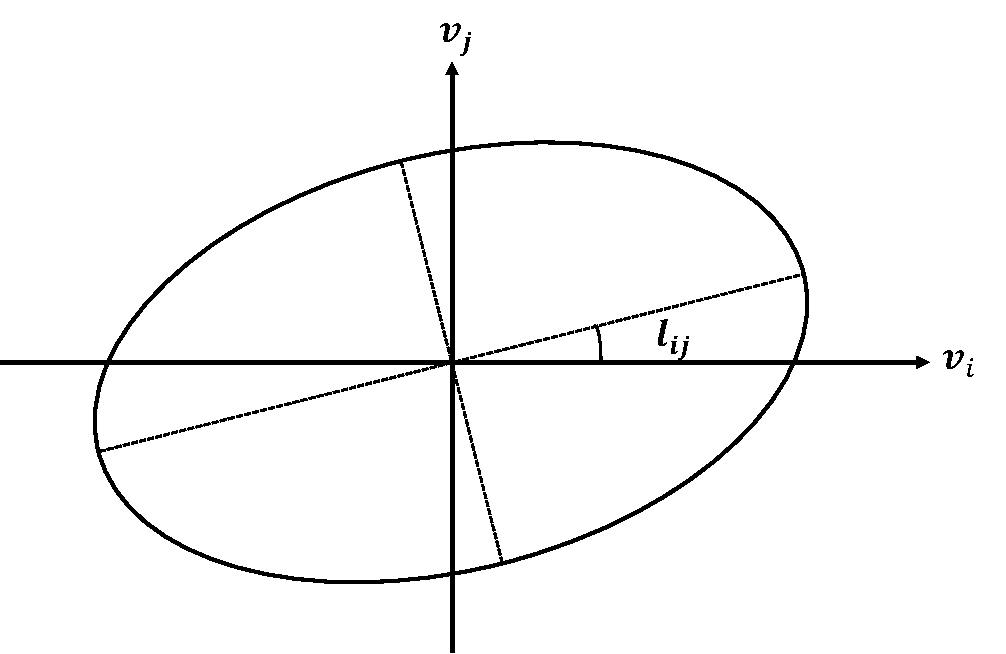
\includegraphics[width=13cm]{fig/velocity_ellipsoid.pdf}
% 	\caption{速度楕円体を2次元に投影したときの図。楕円は速度分散の1$\sigma$にあたる点を結んだ線である。$l_{ij}$は座標軸を図のようにとったときの楕円の主軸との傾きを表す。}
% 	\label{fig:ve}
% \end{figure*}